\section{\'Eléments de théorie de la décision}\label{decision}

L'objectif général de la plupart des études inférentielles est de fournir une \emph{décision} au statisticien (ou au client)
à partir du phénomène modélisé par $X\sim f(x|\theta)$ {(dans le cadre paramétrique)}. Il faut donc exiger un \emph{critère d'évaluation} des procédures de décision qui :
\begin{itemize}
\item prenne en compte les conséquences de chaque décision
\item dépende des paramètres $\theta$ du modèle, càd du \emph{vrai état du monde (ou de la nature)}.
\end{itemize}
 Un autre type de décision est d'{\it évaluer} si un nouveau modèle descriptif est compatible avec les données expérimentales disponibles (\emph{choix de modèle}). Le critère en question est habituellement nommé \emph{\bf fonction de co\^ut}, {\bf fonction de perte} ou \emph{\bf utilité} (opposé du co\^ut). \\

\begin{exo}
Acheter des capitaux selon leurs futurs rendement $\theta$, déterminer si le nombre $\theta$ des SDF a augmenté depuis le dernier recensement... \\
\end{exo}


 
 Formellement, pour le modèle $X\in\{\Omega,{\cal{B}},\{\Pp_{\theta}, \ \theta\in\Theta\}$ on définit donc trois espaces de travail :
 \begin{itemize}
\item $\Omega=$ espace des observations $x$ ;
\item $\Theta=$ espace des paramètres $\theta$ ;
\item ${\cal{D}}=$ espace des décisions possibles $d$.
\end{itemize}
En général, la décision $d\in{\cal{D}}$ demande d'évaluer ({\it estimer}) une  \emph{fonction d'intér\^et} $h(\theta)$, avec $\theta\in\Theta$, estimation fondée sur l'observation $x\in\Omega$. On décrit alors ${\cal{D}}$ comme l'ensemble des fonctions de $\Theta$ dans $h(\Theta)$ où $h$ dépend du contexte :
\begin{itemize}
\item si le but est d'estimer $\theta$ alors ${\cal{D}}=\Theta$ ;
\item si le but est de mener un test, ${\cal{D}}=\{0,1\}$.
\end{itemize}

\subsection{Existence d'une fonction de coût}

La \emph{théorie de la décision} suppose alors que : 
\begin{itemize}
\item chaque décision $d\in{\cal{D}}$ peut \^etre évaluée et conduit à une  \emph{récompense} (ou {\it gain}) $r\in{\cal{R}}$
\item \pause l'espace ${\cal{R}}$ des récompenses peut \^etre  \emph{ordonné totalement} :
\begin{description}
\item[(1)]   $r_1 \preceq r_2$ ou $r_2 \preceq r_1$ ;
\item[(2)]   si $r_1\preceq r_2$ et $r_2\preceq r_3$ alors $r_1\preceq r_3$; 
\end{description}
\item \pause   l'espace ${\cal{R}}$ peut \^etre étendu à l'espace ${\cal{G}}$ des distributions de probabilité dans ${\cal{R}}$ ;
\begin{itemize}
\item   {  les décisions peuvent \^etre alors partiellement aléatoires}
\end{itemize}
\item \pause la relation d'ordre $\preceq$ peut \^etre étendue sur les {\bf moyennes} des récompenses aléatoires {  \it (et donc sur les distributions de probabilité correspondantes)} ;
\begin{itemize}
\item    il existe au moins un ordre partiel sur les gains (m\^eme aléatoires) et un gain optimal.
\end{itemize}
\end{itemize}

 Ces axiomes expriment une certaine  \emph{\bf hypothèse de rationalité du décideur}. Ils impliquent l'existence d'une \emph{\bf fonction d'utilité $U(r)$} permettant de trier les gains aléatoires. Cette utilité ne dépend en fait que de $\theta$ et de $d$  : on la note donc 
 $U(\theta,d)$ Elle peut \^etre vue comme une  \emph{mesure de proximité} entre la décision proposée $d$ et la vraie valeur (inconnue) $\theta$. \\
 
 \begin{definition}
 On appelle \emph{fonction de co\^ut} ou \emph{fonction de perte} une fonction $L$ mesurable de $\Theta\times{\cal{D}}$, telle que 
 \begin{eqnarray*}
L(\theta,d) & =  & - U(\theta,d),
\end{eqnarray*}
à valeurs réelles positives : 
$$
L:\Theta\times{\cal{D}} \longrightarrow \R^+.
$$
 \end{definition}
 
La fonction de coût est définie selon le problème étudié et constitue l'armature d'un problème de décision statistique (qui comprend notamment les problèmes d'estimation). \\

\begin{exo}
On considère le problème de l'estimation de la moyenne $\theta$ d'un vecteur gaussien
\begin{eqnarray*}
x & \sim {\cal{N}}_p(\theta,\Sigma)
\end{eqnarray*}
où $\Sigma$ est une matrice diagonale connue avec pour éléments diagonaux $\sigma^2_i$ $(i=1,\ldots,p)$. Dans ce cas ${\cal{D}}=\Theta=\R^p$ et $d$ représente une évaluation de $\theta$. S'il n'y a pas d'information additionnelle disponible sur ce modèle, il para\^it logique de choisir une fonction de co\^ut qui attribue le m\^eme poids à chaque composante, soit un co\^ut de la forme
\begin{eqnarray*}
\sum\limits_{i=1}^p L\left(\frac{x_i - \theta_i}{\sigma_i}\right) \ \ \ \ \text{avec $L(0)=0$}.
\end{eqnarray*}
Par normalisation, les composantes avec une grande variance n'ont pas un poids trop important. Le choix habituel de $L$ est le co\^ut {\bf quadratique} $L(t)=t^2$. \\
\end{exo}

Dans un contexte de gain aléatoire, l' \emph{approche fréquentiste} propose de considérer le  \emph{co\^ut moyen} ou  { \emph{ risque fréquentiste}}. Pour une fonction de coût quadratique, le risque fréquentiste est souvent appelé \emph{risque quadratique}. On appelle  \emph{$\delta:\Omega \mapsto {\cal{D}}$} minimisant un risque un  \emph{ \emph{estimateur}} et  \emph{$\delta(x)$}  une  \emph{ \emph{estimation}}.


\begin{definition}[Risque fréquentiste]
Pour $(\theta,\delta)\in\Theta\times{\cal{D}}$, le risque fréquentiste est défini par
\begin{eqnarray*}
{R(\theta,\delta)} & = &  {\E_{\theta}\left[L(\theta,\delta(x))\right] \ = \ \int_{\Omega} L(\theta,\delta(x)) f(x|\theta) \ dx}
\end{eqnarray*}
où $\delta(x)$ est la règle de décision  = attribution d'une décision connaissant l'observation $x$.
\end{definition}



%\begin{definition}[Estimateur et estimation]

%\end{definition}

\noindent Cette définition du risque n'est pas sans poser problème. En effet :
\begin{itemize}
\item le critère évalue les procédures d'estimation selon leurs  \emph{performances à long terme} et non directement pour une observation donnée ;
\item on suppose tacitement que le problème sera rencontré de nombreuses fois pour que l'évaluation en fréquence ait un sens
\begin{eqnarray*}
R(\theta,\delta) & \simeq & \text{co\^ut moyen sur les répétitions} ;
\end{eqnarray*}
\item ce critère n'aboutit pas à un  \emph{ordre total} sur les procédures de construction d'estimateur. \\
\end{itemize}

\begin{exec}\label{exo6}
Soient $x_1 $ et $x_2$ deux observations de la loi définie par \begin{eqnarray*}
P_{\theta}(x=\theta-1) & = & P_{\theta}(x=\theta+1) \ = \ 1/2 \ \ \ \ \text{avec $\theta\in\R$}
\end{eqnarray*}
Le paramètre d'intér\^et est $\theta$ (donc ${\cal{D}}=\Theta$) et il est estimé par $\delta$ sous le co\^ut
\begin{eqnarray*}
L(\theta,\delta) & = & 1 - \1_{\theta}(\delta)
\end{eqnarray*}
appelé  \emph{co\^ut 0-1}, qui pénalise par 1 toutes les erreurs d'estimation quelle que soit leur magnitude (grandeur). Soit les estimateurs
\begin{eqnarray*}
\delta_1(x_1,x_2) & = & \frac{x_1+x_2}{2}, \\
\delta_2(x_1,x_2) & = & x_1 + 1, \\
\delta_3(x_1,x_2) & = & x_2 - 1. 
\end{eqnarray*}
Calculez les risques $R(\theta,\delta_1)$, $R(\theta,\delta_2)$ et $R(\theta,\delta_3)$. Quelle conclusion en tirez-vous ? 
\end{exec}
\if\mycmdexo1 \begin{rep} %[Exercice \ref{exo6}]
Calculons le risque fréquentiste pour $\delta_1$. On obtient :
\begin{eqnarray*}
R(\theta,\delta_1) & = & \E_{\theta}\left[L(\theta,\delta_1(X))\right], \\
& = & \int_{\Omega} L(\theta,\delta_1(x)) f(x|\theta) \ dx.
\end{eqnarray*}
La fonction $L(\theta,\delta_1(x))$ vaut 0 si $\delta=\theta$ (bonne décision) et 1 sinon. On en déduit que 
\begin{eqnarray*}
R(\theta,\delta_1) & = & \int_{\{\theta-1,\theta+1\}} \left(1-\1_{\theta}((x_1+x_2)/2\right) f(x_1,x_2|\theta) \ dx_1 d x_2, \\
& = & \frac{1}{4}\left\{\left(1-\1_{\theta}((\theta-1+\theta-1)/2)\right) + \left(1-\1_{\theta}((\theta+1+\theta-1)/2)\right) + \right. \\
& & \ \left. \ \left(1-\1_{\theta}((\theta+1+\theta+1)/2)\right) + \left(1-\1_{\theta}((\theta-1+\theta+1)/2)\right)\right\}, \\
& = & \frac{1}{4}(1+1) \ = \ 1/2.
\end{eqnarray*}
(l'estimateur est correct la moitié du temps). 
On trouve alors, similairement,
\begin{eqnarray*}
R(\theta,\delta_1) & = & R(\theta,\delta_2) \ = \ R(\theta,\delta_3) \ = \ 1/2
\end{eqnarray*}
ce qui signifie qu'on ne peut pas classer les estimateurs sous le coût fréquentiste 0-1.
\end{rep}
\fi

\vspace{1cm}

L'approche bayésienne de la théorie de la décision considère que  \emph{le co\^ut $L(\theta,d)$ doit plut\^ot \^etre moyenné sur tous les états de la nature possibles}. Conditionnellement à l'information $x$ disponible, ils sont décrits par la loi {\it a posteriori} $\pi(\theta|x)$. On définit donc le  { { co\^ut moyenné {\it a posteriori}}}, ou \emph{risque a posteriori}, qui est l'erreur moyenne résultant de la décision $d$ pour un $x$ donné. 

\begin{definition}[Risque {\it a posteriori}]
\begin{eqnarray*}
{R_P(d|\pi,x)} & = & {\int_{\Theta} L(\theta,d) \pi(\theta|x) \ d\theta}.
\end{eqnarray*}
\end{definition}

On peut enfin définir le  risque fréquentiste intégré sur les valeurs de $\theta$ selon leur distribution {\it a priori}. Associant un nombre réel à chaque estimateur $\delta$, ce risque induit donc une  \emph{relation d'ordre total}
 sur les procédures de construction d'estimateur. Il permet donc de définir la notion d'estimateur bayésien (ou estimateur de Bayes). 


\begin{definition}[Risque intégré]
\`A fonction de coût (perte) donnée, le risque intégré est défini par
\begin{eqnarray*}
{R_B(\delta|\pi)} & = & {\int_{\Theta} \int_{\Omega} L(\theta,\delta(x)) f(x|\theta) \ dx \ \pi(\theta) \ d\theta}.
\end{eqnarray*}
\end{definition}

\begin{definition}[Estimateur bayésien et risque de Bayes]
Un  \emph{estimateur de Bayes} associé à une distribution {\it a priori} $\pi$ et une fonction de co\^ut $L$ est défini par 
\begin{eqnarray*}
\delta^{\pi} & = & \arg\min\limits_{\delta\in{\cal{D}}} R_B(\delta|\pi)
\end{eqnarray*}
la valeur $r(\pi) = R_B(\delta^{\pi}|\pi)$ est alors appelée  { \emph{\bf risque de Bayes}}.
\end{definition}

\noindent Le résultat suivant peut être obtenu par interversion d'intégrales (théorème de Fubini). {\it Modulo} un peu de machinerie technique, on peut montrer que celui-ci reste vrai m\^eme si $\int_{\Theta}\pi(\theta) d \theta=\infty$ {(mesure {\it a priori} non informative)} à condition que
$\int_{\Theta}\pi(\theta|x) d \theta = 1$. 

\begin{theorem}
Pour chaque $x\in\Omega$,
\begin{eqnarray}
\delta^{\pi}(x) & = & \arg\min\limits_{d\in{\cal{D}}}  R_P(d|\pi,x). \label{risque.bayes.calcul}
\end{eqnarray}
Un corollaire est le suivant : s'il existe $\delta\in{\cal{D}}$ tel que $R_B(\delta|\pi)<\infty$, et si $\forall x\in \Omega$ l'équation (\ref{risque.bayes.calcul}) est vérifiée, alors $\delta^{\pi}(x)$ est un estimateur de Bayes.
\end{theorem}

\if\mycmdproof1 \begin{proof}%[Preuve] % Minimisation estimateur de Bayes via Fubini
Nous prouvons ici qu'un estimateur minimisant le risque intégré $R_B$ est obtenu par sélection, pour chaque valeur $x\in\Omega$, de la valeur $\delta(x)$ qui minimise le coût moyen {\it a posteriori}. Il s'agit en pratique d'une méthode de calcul d'un estimateur bayésien. En effet,
%\begin{eqnarray*}
%R_B(\delta|\pi) & = & \int_{\Omega} R_P(\delta(x)|\pi,x) m_{\pi}(x) \dx.
%\end{eqnarray*}
L'application du théorème de Fubini est possible par la finitude des intégrales impliquées ci-dessous : avec $L(\theta,\delta(x))\geq 0$, il vient
\begin{eqnarray*}
R_B(\delta|\pi) & = & \int_{\Theta}\int_{\Omega} L(\theta,\delta(x)) f(x|\theta) \ dx \pi(\theta) \ d\theta, \\
&= & \int_{\Omega} \int_{\Theta} L(\theta,\delta(x)) f(x|\theta) \pi(\theta) \ d\theta dx, \\
& = & \int_{\Omega} \int_{\Theta} L(\theta,\delta(x)) \pi(\theta|x) \ d\theta m_{\pi}(x) \ dx, \\
& = & \int_{\Omega} R_P(\delta|\pi,x) m_{\pi}(x) \ dx.
\end{eqnarray*}
On peut en déduire que pour tout $\delta\in{\cal{D}}$, 
%\begin{eqnarray*}
$R_P\left(\delta^{\pi}(x)|\pi,x\right)  \leq  R_P\left(\delta|\pi,x\right)
$%\end{eqnarray*}
implique
%\begin{eqnarray*}
$R_B\left(\delta^{\pi}|\pi\right)  \leq  R_B\left(\delta|\pi\right)
$%\end{eqnarray*}
ce qui permet de conclure la démonstration du corollaire.
 \end{proof}
\fi

\vspace{1cm}



\subsection{Supériorité des estimateurs de Bayes sur les estimateurs fréquentistes}

Le risque minimax est le {co\^ut fréquentiste minimum dans le cas le moins favorable} (l'écart entre $\theta$ et $\delta$, càd l'{\it erreur d'estimation}, est maximal(e)).

\begin{definition}[Risque minimax]
On définit le  \emph{ \emph{risque minimax}} pour la fonction de co\^ut $L$ par
\begin{eqnarray*}
\bar{R} & = & \inf\limits_{\delta\in{\cal{D}}}  \sup\limits_{\theta\in\Theta} R(\theta,\delta) \ = \ \inf\limits_{\delta\in{\cal{D}}}  \sup\limits_{\theta\in\Theta} \E_{\theta}\left[L(\theta,\delta(x))\right].
\end{eqnarray*}
\end{definition}

\begin{theorem}
Le risque de Bayes est toujours plus petit que le risque minimax
\begin{eqnarray*}
 \emph{R} = \sup\limits_{\pi} r(\pi) = \sup\limits_{\pi} \inf\limits_{\delta\in{\cal{D}}} R_B(\delta|\pi) & \leq  \bar{R}.
\end{eqnarray*}
\end{theorem}

Si elle existe, une distribution {\it a priori} $\pi^*$ telle que $r(\pi^*)= \emph{R}$ est appelée  \emph{\it distribution a priori la moins favorable}. Ainsi, l'apport d'information {\it a priori} $\pi(\theta)$ ne peut qu'améliorer l'erreur d'estimation, m\^eme dans le pire des cas. \\

\begin{definition}[Inadmissibilité d'un estimateur]\label{inadmin}
Un estimateur $\delta_0$ est dit  \emph{inadmissible} s'il existe un estimateur $\delta_1$ qui {\bf domine} $\delta_0$ au sens du risque fréquentiste, càd si 
\begin{eqnarray*}
R(\theta,\delta_0) & \geq & R(\theta,\delta_1) \ \ \ \ \forall \theta\in\Theta
\end{eqnarray*}
et $\exists \theta_0$ tel que $R(\theta_0,\delta_0) > R(\theta_0,\delta_1)$. Sinon, il est dit  \emph{admissible}.
\end{definition}

%On peut montrer que s'il existe un unique estimateur minimax, alors il est admissible. 

\begin{theorem}
Si un estimateur de Bayes $\delta^{\pi}$ associé à une mesure {\it a priori} $\pi$ (probabiliste ou non) est tel que le risque $R(\theta,\delta^{\pi})<\infty$ et si la fonction $\theta\mapsto R(\theta,\delta)$ est continue sur $\Theta$, alors $\delta^{\pi}$ est admissible.
\end{theorem}


\if\mycmdproof1 \begin{proof}%[Preuve] % Admissibilité d'un estimateur bayésien
Soit un estimateur bayésien $\delta^{\pi}$ de risque $R$ fini. Pour $\delta_0\in{\cal{D}}$ tel que $\forall\theta\in\Theta$, $R(\theta,\delta)\leq R(\theta,\delta_0)$, on note
\begin{eqnarray*}
{\cal{A}}_0 & = & \left\{\theta\in\Theta, \ R(\theta,\delta) \leq R(\theta,\delta_0) \right\}.
\end{eqnarray*}
On a alors
\begin{eqnarray*}
\int_{\Theta} R(\theta,\delta_0) d\Pi(\theta) - \int_{\Theta} R(\theta,\delta^{\pi}) d\Pi(\theta)& = & \int_{{\cal{A}}_0} \left(R(\theta,\delta)-R(\theta,\delta_0)\right)  d\Pi(\theta) \ \leq\ 0 
\end{eqnarray*}
avec égalité si et seulement si $\pi({\cal{A}}_0)=0$. Or, comme $\delta^{\pi}$ est bayésien et le risque fini, $R(\theta,\delta_0)\geq R(\theta,\delta^{\pi})$. Donc l'intégrale ci-dessus est négative et positive, donc nulle, ce qui sous-entend qu'en effet $\pi({\cal{A}}_0)=0$ (on dit alors que $\delta^{\pi}$ est $\pi-$admissible). Supposons cependant que $\delta^{\pi}$ n'est pas admissible. On  déduit de la démarche précédente que  $\exists\delta_0$ tel que $\forall \theta$ tel que $R(\theta,\delta_0)\leq R(\theta,\delta^{\pi})$ et $\theta_0\in\Theta$ tel que $R(\theta,\delta_0) < R(\theta,\delta^{\pi})$. La fonction définie sur $\Theta$ par $\theta\to R(\theta,\delta_0)-R(\theta,\delta^{\pi})$ est continue par hypothèse. Donc il existe un voisinage  ouvert $V_0\subset\Theta$ de $\theta_0$ tel que $\forall \theta\in V_0$, $R(\theta,\delta_0)<R(\theta,\delta^{\pi})$. On a  $\pi({\cal{A}}_0)\geq \pi(V_0)$. Or $\pi$ est supposé strictement positive sur $\Theta$, donc $\pi(V_0)>0$. L'ensemble ${\cal{A}}_0$ est donc de mesure non nulle, ce qui contredit la première partie de la démonstration. En conclusion, $\delta^{\pi}$ est admissible. 
\end{proof}
\fi


\begin{theorem}
Si un estimateur de Bayes $\delta^{\pi}$ associé à une mesure {\it a priori} $\pi$ (probabiliste ou non) et une fonction de coût $L$ est unique, alors il est admissible.
\end{theorem}

\if\mycmdproof1  
 \begin{proof}%[Preuve] % Admissibilité d'un estimateur bayésien
 
Supposons que $\delta^{\pi}$ est non admissible. Alors, d'après la Définition \ref{inadmin}, $\exists \delta_0\in{\cal{D}}$ tel que $\forall \theta\in\Theta$, $R(\theta,\delta^{\pi})\geq R(\theta,\delta_0)$, et  $\exists \theta_0\in\Theta$ tel que $R(\theta_0,\delta^{\pi})>R(\theta_0,\delta_0)$. En intégrant la première inégalité, il vient :
\begin{eqnarray*}
\int_{\Theta} R(\theta,\delta_0) \ d\Pi(\theta) & \leq & \int_{\Theta} R(\theta,\delta^{\pi}) \ d\Pi(\theta) \ = \ R_B(\delta|\pi)
\end{eqnarray*}
donc $\delta_0$ est aussi un estimateur bayésien associé à $L$ et $\pi$, et $\delta_0\neq \delta^{\pi}$ d'après la seconde inégalité. Ce qui contredit à l'hypothèse du théorème. Par contraposée, on en déduit le résultat de ce thèorème. Remarquons que l'unicité de l'estimateur impliqué la finitude du risque :
\begin{eqnarray*}
\int_{\Theta} R(\theta,\delta^{\pi}) \ d\Pi(\theta) & < & \infty
\end{eqnarray*}
sinon tout estimateur minimise le risque.
\end{proof}
\fi


Notons que les critères de minimaxité et d'admissibilité sont éminement  \emph{fréquentistes} (car construits à partir du risque fréquentiste). Selon ces critères fréquentistes, les estimateurs de Bayes font mieux ou au moins aussi bien que les estimateurs fréquentistes :
\begin{itemize}
\item leur risque minimax est toujours égal ou plus petit ;
\item ils sont tous admissibles (si le risque de Bayes est bien défini).
\end{itemize}

Les estimateurs de Bayes, plus généralement, sont souvent optimaux pour les concepts fréquentistes d'optimalité et devraient donc \^etre utilisés m\^eme lorsque l'information {\it a priori} est absente. On peut ignorer la signification d'une distribution {\it a priori} tout en obtenant des estimateurs corrects d'un point de vue fréquentiste. 

\subsection{Choix d'une fonction de coût}

La fonction de co\^ut $L$ est l'élément fondamental du choix d'un estimateur. Le choix dépend du contexte décisionnel et s'écrit souvent sous la forme
\begin{eqnarray*}
L & = & \text{Co\^ut financier, etc.} - \text{Bénéfice}.
\end{eqnarray*}
Une alternative, lorsqu'il est difficile de la construire, est de faire appel à des  \emph{fonctions de co\^ut usuelles, mathématiquement simples et de propriétés connues}. L'idée est simplement de construire une ``distance" usuelle entre $\theta\in\Theta$ et $d\in{\cal{D}}$ permettant une bonne optimisation (convexe par exemple). \\

\begin{exo}{\bf Fonction de coût quadratique}
Soit ${\cal{D}}=\Theta$. On pose
\begin{eqnarray}
L(\theta,\delta) & = & \|\theta-\delta\|^2. \label{cout.quad}
\end{eqnarray}
\end{exo}

Cette fonction de coût constitue le critère d'évaluation le plus commun. Elle est convexe (mais pénalise très (trop) fortement les grands écarts peu vraisemblables). Elle est justifié par sa simplicité, le fait qu'elle permet de produire des estimateurs de Bayes intuitifs, et qu'elle peut \^etre vue comme issue d'un développement limité d'un co\^ut symétrique complexe.


\begin{proposition}\label{prop1}
L'estimateur de Bayes associé à toute loi {\it a priori} $\pi$ et au co\^ut (\ref{cout.quad}) est l'espérance (moyenne) de la loi {\it a posteriori} $\pi(\theta|{\bf x_n})$
\end{proposition}
\if\mycmdproof1 \begin{proof}%[Preuve] % Espérance a priori
On a ${\cal{D}}=\Theta\in\R^d$ (ou plus généralement un espace de Hilbert) et $L(\theta,\delta)=\|\theta-\delta\|^2$ (norme euclidienne au carré). Par simplificité travaillons sur $\Theta=\R$ (d=1). Alors
\begin{eqnarray*}
R_{P}\left(\delta|\pi\right) & = & \int_{\Theta} (\theta-\delta)^2 \pi(\theta|x) \ d\theta, \\
& = & \E[\theta^2|x] - 2\delta\E[\theta|x] + \delta^2.
\end{eqnarray*}
En dérivant en $\delta$, on obtient 
\begin{eqnarray*}
R'_{P}\left(\delta|\pi\right) & = & 2\delta-2\E[\theta|x]
\end{eqnarray*}
valant 0 en $\delta=\E[\theta|x]$. Or
\begin{eqnarray*}
R''_{P}\left(\delta|\pi\right) & = & 2 \ > \ 0
\end{eqnarray*}
donc  $\delta\to R_{B}\left(\delta|\pi\right)$ est convexe, ce qui signifie que la solution de $R'_{P}\left(\delta|\pi\right)=0$ est bien un minimisateur du risque. 
 \end{proof}
\fi

\vspace{0.5cm}

La fonction de coût absolu, également convexe, croît plus lentement que le coût quadratique et ne surpénalise pas les erreurs grandes et peu vraisemblables.  \\

\begin{exo}{\bf Fonction de coût absolu (Laplace 1773)}
Soit ${\cal{D}}=\Theta$ et $\dim\Theta=1$. On pose
\begin{eqnarray}
L(\theta,\delta) & = & |\theta-\delta| \label{cout.abs}
\end{eqnarray}
ou plus généralement une fonction linéaire par morceaux 
\begin{eqnarray}
L_{c_1,c_2}(\theta,\delta) & = & \left\{\begin{array}{ll} c_2(\theta-\delta) & \text{si $\theta>\delta$} \\ c_1(\delta-\theta) & \text{sinon} 
\end{array} \right. \label{cout.lin}
\end{eqnarray}
\end{exo}

\begin{proposition}\label{prop2}
L'estimateur de Bayes associé à toute loi {\it a priori} $\pi$ et au co\^ut (\ref{cout.lin}) est le fractile $c_1/(c_1+c_2)$ de la loi {\it a posteriori} $\pi(\theta|{\bf x_n})$. En particulier, la médiane de la loi {\it a posteriori} est l'estimateur de Bayes lorsque $c_1=c_2$ (qui sont donc des co\^uts associés à la sous-estimation et la surestimation de $\theta$).
\end{proposition}
\if\mycmdproof1 \begin{proof}%[Preuve] % Fonction de coût L1
Considérons la situation générique où 
\begin{eqnarray}
L_{c_1,c_2}(\theta,\delta) & = & \left\{\begin{array}{ll} c_2(\theta-\delta) & \text{si $\theta>\delta$} \\ c_1(\delta-\theta) & \text{sinon} 
\end{array} \right. \label{cout.lin}
\end{eqnarray}
Le risque {\it a posteriori} s'écrit
\begin{eqnarray*}
R_P(\delta|\pi) & = & \int_{-\infty}^\delta c_1(\delta-\theta)\pi(\theta|x) \ d\theta +  \int_{\delta}^{\infty} c_2(\theta-\delta)\pi(\theta|x) \ d\theta.
\end{eqnarray*}
En raisonnant par intégration par parties (IPP), il vient :
\begin{eqnarray*}
R_P(\delta|\pi) & = & \left[c_2(\theta-\delta) \Pi(\theta|x)\right]^{\delta}_{-\infty} + c_2 \Pi(\theta<\delta|x) +   
\left[c_1(\delta-\theta) \Pi(\theta\right]^{\infty}_{\delta} - c_1\Pi(\theta>\delta|x), \\
& = & c_2 \Pi(\theta<\delta|x) + c_1\left(1-\Pi(\theta<\delta|x)\right)
\end{eqnarray*}
car $\lim_{\theta\to-\infty} \Pi(\theta\x) = \lim_{\theta\to\infty} \Pi(\theta\x) = 0$. 
Ce risque est minimum lorsque $R_P(\delta|\pi)=0$ soit lorsque
\begin{eqnarray*}
\Pi(\theta<\delta^{\pi}|x) & = & \frac{c_1}{c_1+c_2}
\end{eqnarray*}
 ce qui confère donc à l'estimateur $\delta^{\pi}$ le sens du quantile de seuil  $\frac{c_1}{c_1+c_2}$.
\end{proof}
\fi

La fonction de coût 0-1, non quantitative, est utilisé dans l'approche statistique classique pour construire des test d'hypothèse. \\

\begin{exo}{\bf Fonction de coût 0-1}
\begin{eqnarray}
L(\theta,\delta) & = & \left\{\begin{array}{ll} 1-\delta & \text{si $\theta\in\Theta_0$} \\ \delta & \text{sinon} \end{array}\right. \label{cout01}
\end{eqnarray}
Le risque fréquentiste associé est 
\begin{eqnarray*}
R(\theta,\delta) & = & \E_{\theta}[L(\theta,\delta(x))] \ = \ \left\{\begin{array}{ll} P_{\theta}(\delta(x)=0) & \text{si $\theta\in\Theta_0$} \\ P_{\theta}(\delta(x)=1) & \text{sinon} \end{array}\right.
\end{eqnarray*}
\end{exo}

\begin{proposition}\label{prop3}
L'estimateur de Bayes associé à toute loi {\it a priori} $\pi$ et au co\^ut 0-1 est 
\begin{eqnarray*}
\delta^{\pi} & = & \left\{\begin{array}{ll} 1 & \text{si $\Pi(\theta\in\Theta_0|{\bf x_n}) > \Pi(\theta\notin\Theta_0|{\bf x_n})$} \\ 0 & \text{sinon} \end{array}\right. \label{cout01}
\end{eqnarray*}
\end{proposition}
\if\mycmdproof1 \begin{proof}%[Preuve] % Fonction de coût 0-1
 Cette fonction de perte est utilisée dans le contexte des tests statistiques. On suppose partitionner $\Theta$ en $\Theta_0$ et $\Theta_1$. La fonction de perte correspondante est alors
 \begin{eqnarray*}
 L(\theta,\delta) & = & \1_{\theta\in\Theta_0} \1_{\delta=1} + \1_{\theta\in\Theta_1} \1_{\delta=0}.
 \end{eqnarray*}
 Le risque {\it a posteriori} est alors
 \begin{eqnarray*}
 R_P(\delta|\pi) & = & \1_{\delta=1} \Pi(\theta\in\Theta_0|x) + \1_{\delta=0} \Pi(\theta\in\Theta_0|x). 
 \end{eqnarray*}
 Ainsi $\delta^{\pi}=1$ équivaut à $\Pi(\theta\in\Theta_0|X)\leq \Pi(\theta\in\Theta_1|X)$.
\end{proof}
\fi
 
 
 \vspace{0.5cm}

Ainsi, l'estimation bayésienne permet d'accepter une hypothèse (nulle) $H_0:$ $\theta\in\Theta_0$, si c'est l'hypothèse la plus probable {\it a posteriori}, ce qui est une réponse intuitive. \\




Une variante du test 0-1 est le test de Neyman-Pearson qui permet de distinguer risques de première et de deuxième espèce :
\begin{eqnarray}
L(\theta,d)  =  \left\{\begin{array}{ll} 0 & \text{si $d=\I_{\Theta_0}$} \\ a_0 & \text{si $\theta\in\Theta_0$ et $d=0$} \\ a_1 & \text{si $\theta\notin\Theta_0$ et $d=1$} \end{array}\right. &  & \label{cout.generalise}
\end{eqnarray}
qui donne l'estimateur bayésien
\begin{eqnarray*}
\delta^{\pi}(x)  =  \left\{\begin{array}{ll} 1 & \text{si $\Pi(\theta\in\Theta_0|x) > a_1/(a_0+a_1)$,} \\ 0 & \text{sinon.} \end{array}\right. 
\end{eqnarray*}
Ainsi, l'hypothèse nulle est rejetée quand la probabilité {\it a posteriori} de $H_0$ est trop petite. Il est cependant délicat de choisir les poids $a_0$ et $a_1$ sur des considérations d'utilité. \\

 Plus généralement, ce résultat permet d'illustrer une différence majeure entre statistique classique et statistique bayésienne. L'approche classique (dite de Fisher-Neyman-Pearson) suppose qu'on puisse définir une statistique de test dont la loi, sous l'hypothèse nulle $H_0$, est indépendante du paramètre estimé sous $H_0$. Ce faisant, la seule décision que l'on peut prendre avec une bonne certitude est de refuser $H_0$. Cette dissymétrie entre $H_0$ et toute autre hypothèse alternative $H_1$ n'existe pas dans le cadre bayésien : celui-ci émet un prior sur chaque modèle en compétition, puis compare les modèles selon leur probabilité d'explication des données disponibles {\it a posteriori}. Cette approche semble plus séduisante d'un point de vue intuitif et opérationnel. Voir également $\S$ \ref{test} pour plus de détails.


\subsection{Coûts intrinsèques}

On peut enfin chercher à à trouver des fonctions de co\^uts qui restent invariantes par \emph{transformation monotone inversible} sur les données (action d'un $C^1-$difféomorphisme sur $\Omega$). On obtient ce faisant des fonctions de co\^uts définies à partir de \emph{distances}  ou de \emph{divergences} $D$ entre distributions 
\begin{eqnarray*}
L(\theta,d) & = & D(f(.|\theta) \ \| \ f(.|d)). 
\end{eqnarray*}
Ci-dessous, quelques distances ou divergences usuelles entre des densités $(f_{\theta},f_{\theta'})$ de fonctions de répartition $(F_{\theta},F_{\theta'})$, qui induisent des fonctions de coût intrinsèques, sont présentées. 

\begin{center}
    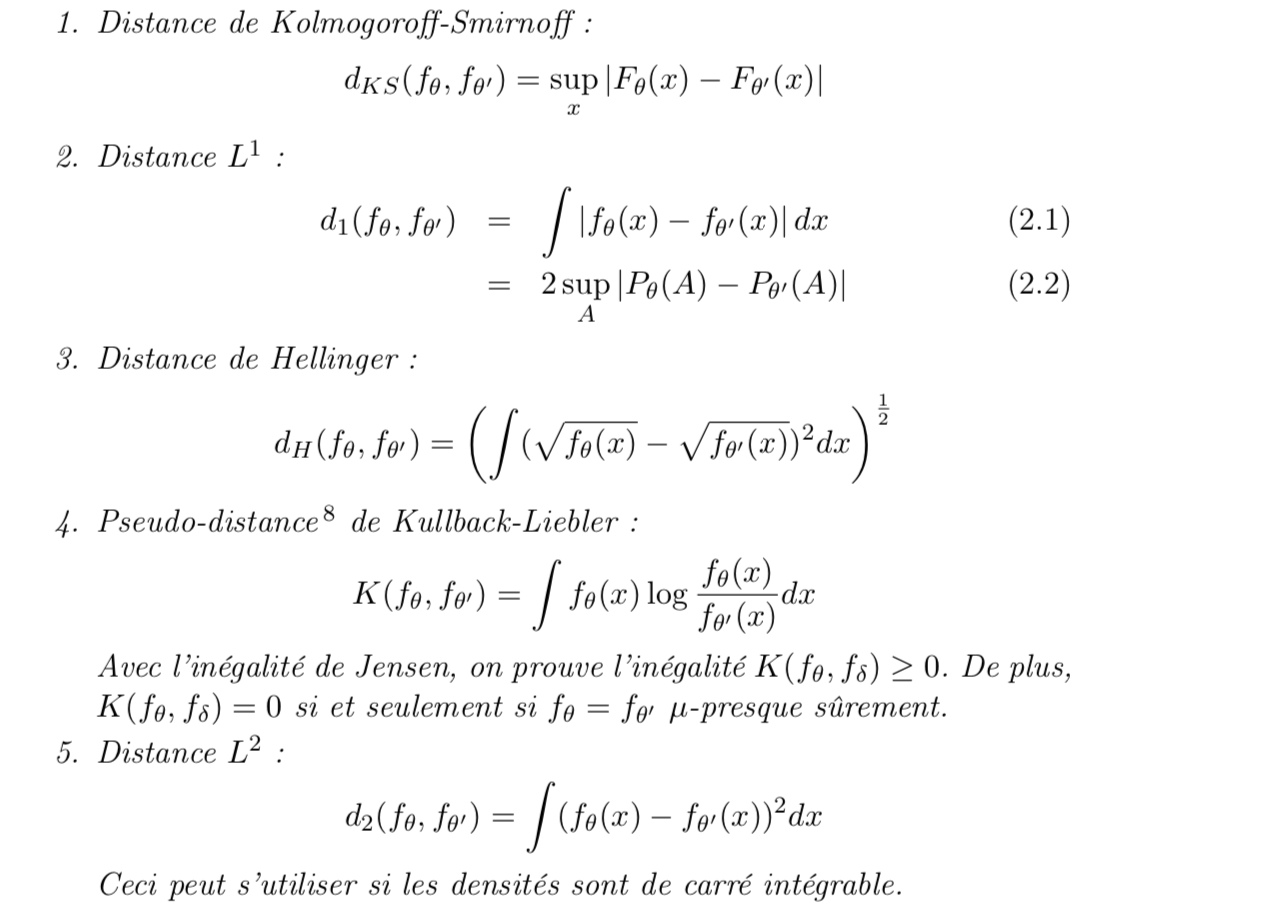
\includegraphics[scale=0.3]{figures/metrics-intrinsic}
\end{center}

\subsubsection*{Rappels sur la divergence de Kullback-Leibler (KL)}\label{rappels.KL}

La divergence KL a un sens issu de la théorie de l'information (qui sera rappelé plus loin dans le cours). Rappeler ses principales propriétés peut être utile. Soit $\pi_1(\theta)$ et $\pi_2(\theta)$ deux densités de probabilité définies sur un même espace $\Theta$, $\pi_1$ étant absolument continue par rapport à $\pi_2(\theta)$. Alors
\begin{eqnarray*}
\mbox{KL}(\pi_1 || \pi_2) & = & \E_{\pi_1}\left[\log\frac{\pi_1(\theta)}{\pi_2(\theta)}\right], \\
& = & \int_{\Theta} \pi_1(\theta) \log\frac{\pi_1(\theta)}{\pi_2(\theta)} \ d\theta.
\end{eqnarray*}

\begin{proposition} Si $\pi_1(\theta)$ et $\pi_2(\theta)$ sont propres, alors 
$\mbox{KL}(\pi_1 || \pi_2)\geq 0$ et vaut 0 si et seulement si $\pi_1=\pi_2$ (presque partout)
\end{proposition}

La preuve de ce résultat est fondée sur l'application de l'inégalité de Jensen à la fonction $\pi_1\to \pi_1\log \pi_1$, qui est différentiable deux fois sur l'espace des densités de probabilités, et dont la différentielle seconde vaut $1/\pi_1>0$. Elle est donc convexe. Alors  $\mbox{KL}(\pi_1 || \pi_2)\geq - \log 1 = 0. 



\begin{exec}
Lorsqu'on fait un choix de fonction de coût $L(\theta,\delta)$ dans un ensemble $U:\Theta\times{\cal{D}}\to\Lambda\in\R^+$, on commet une erreur par rapport à la meilleure fonction de coût possible pour le problème. On peut donc proposer un estimateur bayésien de cette fonction de coût en introduisant une fonction de coût sur les fonctions de coût $L(\theta,\delta)$ :
\begin{eqnarray*}
\tilde{L}: \Theta\times U \times {\cal{D}}  & \to & \R^+ \\
(\theta,\ell,\delta) & \mapsto & \tilde{L}(\theta,\ell,\delta).
\end{eqnarray*}
Quel est l'estimateur bayésien de $\tilde{L}(\theta,\ell,\delta)$ sous un coût quadratique, lorsque $L(\theta,\delta)$ est elle-même quadratique ?
\end{exec}

\if\mycmdexo1 \begin{rep} % Fonction de coût sur les fonctions de coût
Si $\tilde{L}(\theta,\ell,\delta)=(\ell-L(\theta,\delta))^2$ et $L(\theta,\delta)=(\theta-\delta)^2$, alors l'estimateur bayésien est
\begin{eqnarray*}
\ell^{\pi}  & = & \E_{\pi}\left[L(\theta,\delta)|X \right] \\
& = &  \E_{\pi}\left[(\theta-\delta)^2|X\right].
\end{eqnarray*}
En choisissant en toute logique $\delta=\delta^{\pi}=\E[\theta|X]$ il vient donc
$$
\ell^{\pi}  = \mbox{Var}_{\pi}[\theta|X].
$$
\end{rep}
\fi




\subsection{Mode {\it a posteriori} (MAP)}

L'estimateur du  mode {\it a posteriori}, ou MAP, est défini par
\begin{eqnarray*}
\delta^{\pi}({\bf x_n}) & = & \arg\max\limits_{\theta\in\Theta} \pi(\theta|{\bf x_n}).
\end{eqnarray*}
Cet estimateur, contrairement aux précédents, n'est pas issu de la minimisation d'une fonction de coût (il n'est donc pas bayésien {\it stricto sensu}) mais peut être vu comme la limite d'estimateurs bayésiens. \\

Il correspond à un maximum de vraisemblance (MV) pénalisé (voir $\S$ \ref{estimation.MAP.ML}) et souffre donc en général des mêmes  inconvénients que le MV, en particulier une certaine instabilité d'estimation ponctuelle. Par ailleurs, à la différence du MV, il est en général non invariant par reparamétrisation. Cette gêne décisionnelle mène à le déconseiller formellement, ou du moins à s'en méfier, même si ce type d'estimateur est couramment privilégié par les praticiens du \textit{machine learning}. 


\subsection{Sélection de modèle et facteur de Bayes}\label{test}

La sélection de modèle bayésien est un choix particulier de décision. D'une fa\c con générale, supposons vouloir tester deux hypothèses de modèles, $M_0$ et $M_1$, l'une contre l'autre, et pouvoir assigner à ces modèles des probabilités {\it a priori} non nulles
\begin{eqnarray*}
\Pi(M_0), \ \Pi(M_1)
\end{eqnarray*}
d'expliquer des données $X$ non encore observées. Typiquement, on peut vouloir :
\begin{itemize}
    \item pour un même modèle de vraisemblance $f(X|\theta)$, tester {\it a posteriori} deux sous-ensembles  différents de $\Theta$ : $\Pi(\theta\in\Theta_0|X)>0$ et $\Pi(\theta\in\Theta_1|X)>0$;% :
    %\begin{eqnarray*}
    %\Pi(M_i) & = & \Pi(\theta\in\Theta_i) ;
    %\end{eqnarray*}
    \item plus généralement tester un couple $(f_0(x|\theta_0),\pi_0(\theta_0))$ contre un couple $(f_1(x|\theta_1),\pi_1(\theta_1))$, avec $\theta_i\in\Theta_i$. % : on notera alors
    %\begin{eqnarray*}
    %\Pi(M_i) & = & \Pi(\theta\in\Theta_i) ;
    %\end{eqnarray*}
\end{itemize}
 Le facteur de Bayes est le \emph{rapport de  la vraisemblance marginale} de ces deux hypothèses concurrentes :
 \begin{eqnarray}
 B_{01}(X) & = & \frac{P(X|M_0)}{P(X|M_1)}\label{facteur.bayes}
 \end{eqnarray}
 où 
 \begin{eqnarray*}
 P(X|M_i) & = & \int_{\Theta_1} f_i(X|\theta_i)\pi_i(\theta_i) \ d\theta_i, \\
 & = &   \frac{\Pi(M_i|X) P(X)}{\Pi(M_i)}
 \end{eqnarray*}
 où $P(X)$ représente la loi inconnue des données. Le rapport (\ref{facteur.bayes}) peut alors se simplifier en 
  \begin{eqnarray}
 B_{01}(X) & = & \frac{\Pi(M_0|X) }{\Pi(M_1|X) }\frac{\Pi(M_1)}{\Pi(M_0)}. \label{facteur.bayes.2}
 \end{eqnarray}
 Le {facteur de Bayes} est donc une transformation bijective de la probabilité {\it a posteriori}, qui a fini par \^etre l'outil le plus utilisé pour \textcolor{black}{choisir un modèle bayésien}. Lorsque les deux modèles sont également probables {\it a priori}, alors  $\frac{\Pi(M_1)}{\Pi(M_0)}=1$ et le rapport de Bayes est simplement le rapport de leurs probabilités {\it a posteriori}. \\
 
 
 Le cas le plus fréquemment rencontré en pratique est celui où l'hypothèse de modèle $M_i$ se réduit à $\theta\in\Theta_i$. Il amène à la définition suivante.
 

%Supposons qu'on cherche à mener le test d'une  \textcolor{black}{\it hypothèse nulle $H_0:$ $\theta\in\Theta_0$}.  Soit $H_1: \ \theta\in\Theta_1$ une hypothèse alternative. \\

. 

\begin{definition}
Le \textcolor{black}{facteur de Bayes} associé au problème du choix entre $\theta\in\Theta_0$ et $\theta\in\Theta_1$ est le rapport des probabilités {\it a posteriori} des hypothèses nulle et alternative sur le rapport {\it a priori} de ces m\^emes hypothèses
\begin{eqnarray}
B_{01}(X) & = & \left.\left(\frac{\Pi(\theta\in\Theta_0|X)}{\Pi(\theta\in\Theta_1|X)}\right) \middle/ \left(\frac{\Pi(\theta\in\Theta_0)}{\Pi(\theta\in\Theta_1)}\right)\right. \label{facteur.bayes.3}
\end{eqnarray} 
qui se réécrit comme le \textcolor{black}{pendant bayésien du rapport de vraisemblance} en rempla\c cant les vraisemblances par les \textcolor{black}{marginales} (les vraisemblances intégrées sur les {\it a priori}) sous les deux hypothèses
\begin{eqnarray*}
B_{01}(X) & = & \frac{\int_{\Theta_0} f(X|\theta) \pi_0(\theta) \ d\theta}{\int_{\Theta_1} f(X|\theta) \pi_1(\theta) \ d\theta} \ = \ \frac{f_0(X)}{f_1(X)}
\end{eqnarray*}
\end{definition}

\vs Sous le co\^ut généralisé (\ref{cout.generalise}), en posant
\begin{eqnarray*}
\gamma_0 = \Pi(\theta\in\Theta_0) & \text{et} & \gamma_1 = \Pi(\theta\in\Theta_1).
\end{eqnarray*}
Ainsi l'hypothèse $H_0$ est acceptée si 
$$
B_{01}(x)   >  (a_1\gamma_1)/(a_0\gamma_0).
$$
Dans le pratique, on utilise souvent des échelles logarithmiques pour faire une sélection de modèle (échelle de Jeffreys améliorée par Kass et Raftery) :
\begin{description}
\item[(i)]   si $\Lambda=\log_{10} B_{10}({\bf x_n})$ varie entre 0 et 0.5, la certitude que $H_0$ est {\it fausse est faible} ;
\item[(ii)]  si $\Lambda\in[0.5,1]$, cette certitude est {\it substantielle} ;
\item[(iii)] si $\Lambda\in[1,2]$, elle est {\it forte} ;
\item[(iv)]  si $\Lambda>2$, elle est {\it décisive}.
\end{description}
Malgré le c\^oté heuristique de l'approche, ce genre d'échelle reste très utilisé. \\

\begin{exec}
Soit $X\sim{\cal{B}}(\theta)$ (loi de Bernoulli) avec $\Theta=[0,1]$. Soit $M_0$ un modèle défini par $\{\theta=1/2\}$ et $M_1$ un modèle défini par un $\theta$ inconnu dans $[0,1]$, avec $\pi_1(\theta)={\cal{U}}[0,1]$. Un échantillon de 200 tirages fournit 115 succès et 85 échecs. Au vu de ces données, quel modèle choisir ? Ce résultat diffère-t-il significativement d'un test fréquentiste ?
\end{exec}


\if\mycmdexo1 \begin{rep}% Régions HPD
La vraisemblance des données $X$ est binomiale :
$$
f(x|\theta) = \left(\begin{array}{l} 200 \\ 115 \end{array}\right) \theta^{115}(1-\theta)^{85}
$$
ce qui permet de calculer
\begin{eqnarray*}
P(X|M_0) & = & \left(\begin{array}{l} 200 \\ 115 \end{array}\right) (1/2)^{200} \ \simeq \ 0.006
\end{eqnarray*}
alors que pour $M_1$ on a
\begin{eqnarray*}
P(X|M_1) & = & \int_0^1 \left(\begin{array}{l} 200 \\ 115 \end{array}\right) \theta^{115}(1-\theta)^{85} \ d\theta \ = \ 1/201 \ \simeq \ 0.005.
\end{eqnarray*}
Le facteur de Bayes vaut alors 1.2, ce qui indique uniquement que la certitude que $H_0$ est vraie est faible (on pointe très légèrement vers le modèle $M_0$). 

Un test d'hypothèse fréquentiste de $M_0$ indiquerait que $M_0$ doit être rejeté par exemple au niveau de signification 5\%, car la probabilité d'obtenir 115 succès ou plus à partir d'un échantillon de 200 si $\theta=1/2$ est de 0.02. On en conclut qu'un test classique donnerait des résultats significatifs permettant de rejeter $H_0$ tandis qu'un test bayésien ne pourrait considérer le résultat comme extrême.

\end{rep}
\fi


\begin{remark}
Le calcul du facteur de Bayes n'est pas évident et demande le plus souvent de savoir simuler {\it a posteriori}. \\
\end{remark}

\subsubsection*{Cas de l'estimation ponctuelle et des tests de significativité en régression}

Dans la définition (\ref{facteur.bayes.3}), on sous-entend que chaque alternative $\Pi(\theta\in\Theta_i)>0$ sinon le facteur de Bayes n'est pas défini. Cela exclurait les situations fréquentes où $\Theta_i$ est de mesure nulle. Par exemple lorsqu'on veut tester $\Theta_0=\{\theta_0\}$, ou pour mener un test de significativité pour les modèles de régression. \\

Considérons le cas suivant : on dispose d'un modèle de régression
\begin{eqnarray*}
y & = & \beta_0 + \beta_1 x_1 + \ldots + \beta_d x_d
\end{eqnarray*}
où $\beta_d\in\R$, 
et on veut mener un test de significativité sur $\theta=\beta_d$ :
\begin{eqnarray*}
M_0: \ \{\beta_d = 0\} & vs & M_1: \ \{\beta_d \neq 0\}
\end{eqnarray*}
On peut alors noter $\Theta_0=\{\theta_0\}=\{0\}$ et $\Theta_1=\R^*$. 
Il est clair que  $\Pi(\theta\in\Theta_0)=0$ car la mesure dominante est Lebesgue. Donc la formulation (\ref{facteur.bayes.3}) n'est pas applicable. On peut alors reposer le test en redéfinissant plus généralement
\begin{eqnarray*}
M_0: \ \{|\beta_d-\theta_0| = \epsilon\} & vs & M_0: \ \{|\beta_d| \neq \epsilon\}
\end{eqnarray*}
avec un $\epsilon$ tendant vers 0 par valeurs positives. Reste la difficulté majeure que $\epsilon$ est inconnu et dépend du contexte de l’étude. \\

Plus généralement, et pour mieux formaliser les choses, il convient alors d'introduire une masse de Dirac $\delta_{\theta_0}$ en $\theta_0$ et de considérer un poids $\rho_{\epsilon}\in[0,1]$ à $\epsilon$ fixé, valant \begin{eqnarray*}
\rho_{\epsilon} = \Pi(\theta | |\theta-\theta_0|<\infty) \ = \ \Pi(\theta\in\Theta_0)
\end{eqnarray*}
Le mélange
\begin{eqnarray*}
\pi(\theta) & = & \rho_{\epsilon}\delta_{\theta_0} + (1-\rho_{\epsilon})\pi_1(\theta),
\end{eqnarray*}
désigne la loi {\it a priori} qui généralise $\Pi(\theta\in\Theta_0)$ et $\Pi_1(\theta)=\Pi(\theta\in\Theta_1)$, la densité de cette dernière loi étant absolument continue par rapport à la mesure de Lebesgue.
Dans ce cas, l'application de la formule (\ref{facteur.bayes.3}) donne directement 
\begin{eqnarray*}
B_{01}(X) & = & \frac{\rho_{\epsilon} f(X|\theta_0)}{(1-\rho_{\epsilon})\int_{\theta\in\Theta_1} f(X|\theta) \pi_1(\theta) \ d\theta} \left( \frac{1-\rho_{\epsilon}}{\rho_{\epsilon}}\right), \\
& = & \frac{f(X|\theta_0)}{\int_{\theta\in\Theta_1} f(X|\theta) \pi_1(\theta) \ d\theta}. 
\end{eqnarray*}
(on retrouve bien le rapport des lois marginales). 


\subsubsection*{Cas d'un ou plusieurs priors impropres}\label{priors.impropres.choix}

Une remarque importante concerne le cas où $\pi_0$ ou $\pi_1$ n’est pas un \emph{prior propre} (mesure non intégrable). Dans ce cas, $B_{01}$ n’est alors pas défini de manière unique. En effet, si une loi est impropre (par exemple $\pi_0$) alors elle est définie à une constante multiplicative
près. Pour $\pi^*_0(\theta) = c \pi_0(\theta)$, alors le facteur de Bayes est lui aussi multiplié
par $c$ : $B^*_{01} = c B_{01}$ et par conséquent les ordres de grandeur de $B_{01}$ n’ont 
plus de sens : il n’est plus possible de comparer ses valeurs à une échelle dédiée. \\

\begin{exo}
Soit $X\sim{\cal{N}}(\theta,1)$ et $\pi(\theta)=c\neq 0$. On considère le test suivant : $H_0:\theta=0$ vs $H_1=\theta\neq 0$. Dans ce cas, le facteur de Bayes est
\begin{eqnarray*}
B_{01}(X=x) & = & \frac{\exp(-x^2/2)}{c\sqrt{2\pi}}
\end{eqnarray*}
$c$ étant inconnu, le facteur de Bayes ne peut avoir d'interprétation. \\
\end{exo}

Pour pallier ce problème, des démarches ont été inventées, qui visent à séparer l'échantillon $X$ en sous-échantillons et transformant les priors impropres en posteriors propres (mais faiblement informatifs) : les \emph{facteurs de Bayes fractionnels} ou les \emph{facteurs de Bayes intrinsèques}. Ils ont de bonnes propriétés asymptotiques. Toutefois, dans les dernières années, la recherche se tourne plutôt vers des approches par \emph{mélanges de modèles bayésiens}, qui permettent de remplacer la sélection d'un sous-modèle via le facteur de Bayes par la sélection d'un sous-modèle via les poids du mélange. Ce type d'approche permet de se débarasser, sous certaines conditions, des problèmes posés par les priors impropres.  \\

\begin{exec}{\bf Sélection de modèle discret avec des priors impropres.}
\begin{enumerate}
    \item Pour des données discrètes $x_1,\ldots,x_n$, on considère un modèle de Poisson ${\cal{P}}(\lambda)$ ou une loi binomiale négative ${\cal{NB}}(m,p)$ avec les {\it a priori} 
\begin{eqnarray*}
\pi_1(\lambda) & \propto & 1/\lambda \\
\pi_2(m,p) & = & \frac{1}{M} \1_{\{1,\ldots,M\}}(m) \1_{[0,1]}(p)
\end{eqnarray*}
Peut-on sélectionner l'un des deux modèles ?
\item Si on remplace $\pi_1(\lambda)$ par un {\it a priori} {\bf vague}
$$
\pi_1(\lambda)  \equiv  {\cal{G}}(\alpha,\beta)
$$
avec $\alpha(\beta)$ ou/et $\beta(\alpha) \to 0$, peut-on de nouveau résoudre le problème ? 
\end{enumerate}
\end{exec}

\if\mycmdexothree1 \vspace{1cm} \begin{rep}
\begin{enumerate}
    \item Il existe une constante inconnue $\gamma >0$ telle que %(le donner pour $i=1$, plus simple)
\begin{eqnarray*}
B_{12}({\bf x_n}) & = & \gamma \frac{\int_{0}^{\infty} \frac{\lambda^{\sum_{i} (x_i-1)}}{\prod_i x_i !} \exp\left(-n \lambda\right) \ d\lambda}
{\frac{1}{M}\sum\limits_{m=1}^M \int_{0}{\infty} 
\left(\prod_i\left(\begin{array}{l} m \\ x_i-1\end{array}\right) \right) p^{\sum_i x_i} (1-p)^{m\cdot n - \sum_i x_i} \ dp}, \\
& = & \gamma M\left(\sum_{m=1}^M  \left(\begin{array}{l} m \\ x-1\end{array}\right) \frac{x!(m-x)!}{m!}\right)^{-1} \ \ \text{si $n=1$ et $x_i=x$}\\
& = & \gamma M\left(\sum_{m=1}^M  x/(m-x+1)\right)^{-1}
\end{eqnarray*}
Impossible de faire un choix car $\gamma$ n'est pas connu ! 
\item Si on remplace $\pi_1(\lambda)$ par un {\it a priori} {\bf vague}
$$
\pi_1(\lambda)  \equiv  {\cal{G}}(\alpha,\beta)
$$
avec $\alpha(\beta)$ ou/et $\beta(\alpha) \to 0$, 
on obtient après quelques calculs (pour $n=1$ et $x_i=x$)
\begin{eqnarray*}
B_{12} & = & \frac{\Gamma(\alpha+x)}{x!\Gamma(\alpha)} \beta^{-x}\left[\frac{1}{M}\sum\limits_{m=1}^M \frac{x}{m-x+1}\right]^{-1} \\
& = & \frac{(x+\alpha-1)\ldots \alpha}{x(x-1)\ldots 1} \beta^{-x} \left[\frac{1}{M}\sum\limits_{m=1}^M \frac{x}{m-x+1}\right]^{-1}  
\end{eqnarray*}
qui dépend fortement du choix de $\alpha(\beta)$ ou/et $\beta(\alpha) \to 0$. On ne résout donc pas le problème...
\end{enumerate}
\end{rep}
\fi
\vspace{0.5cm}



%%%%%%%%%%%%%%%%%%% TP avec correction %%%%%%%%%%%%%%%
\clearpage
 \subsection{TP : Création d'un système d'alerte pour la circulation routière}

On s'intéresse à un évènement routier $X=x$ relevé par un système de détection vivant dans l'espace $\chi$ de dimension finie. Ce système de détection peut prédire des évènements répétés du type "un animal sur la voie", "accrochage", "accident", "bouchon"... La question est de déterminer si, à chaque fois qu'un événement routier $x$ est collecté, il est utile qu'une intervention de secours soit menée. \\

Nommons $\theta$ une variable indiquant la gravité de l'évènement. Cette variable a des valeurs dans les ensembles disjoints $\Theta_0$ (incidents sans gravité) et $\Theta_1$   (accidents nécessitant possiblement une intervention). On suppose disposer d'un échantillon labélisé  ${\bf e_n}=({\bf x_n},{\bf \theta_n})$. \\

\paragraph{\bf Questions.} \\
\begin{enumerate}
\item Lorsqu'une observation $x$ apparaît, comment prévoir $\theta$ ?
\item Comment peut-on en déduire une alarme efficace ? 
\end{enumerate}

\if\mycmdtpone1 \paragraph{\bf Réponses.} \\
{\bf 1.} Dans un cadre bayésien, probabilisons l'espace $\Theta= \Theta_0 \oplus \Theta_1$ et nommons $\Pi$ la mesure de probabilité associée. On note également $P$ la mesure de probabilité associée à l'espace $\chi$ supposé probabilisé. On souhaite prévoir la probabilité que $\theta\in\Theta_0$ sachant $x$ et $e_n$. {\it Via} une règle de Bayes, on produit le classifieur classique (dit {\it classifieur de Bayes})
\begin{eqnarray*}
\Pi(\theta\in\Theta_0|x,e_n) & = & \frac{P(X=x|\theta\in\Theta_0,e_n)\Pi(\theta\in\Theta_0|e_n)}{P(X=x|e_n)}, \\
& = & \frac{P(X=x|\theta\in\Theta_0,e_n)\Pi(\theta\in\Theta_0|e_n)}{P(X=x|\theta\in\Theta_0)\Pi(\theta\in\Theta_0|e_n) + P(X=x|\theta\notin\Theta_0)\left[1-\Pi(\theta\in\Theta_0|e_n)\right]}
\end{eqnarray*} 
Le terme de vraisemblance $P(X=x|\theta\in\Theta_0,e_n)$ peut être estimé de nombreuses manières (ex : par  la fréquence d'observation de l' évènement $X=x$ dans les situations recensées pour lesquelles $\theta\in\Theta_0$). Le classifieur de Bayes {\it naïf} repose ainsi sur une simplification de cette vraisemblance, etc. (voir cours d'apprentissage statistique). \\

\vspace{1cm}

{\bf 2.}  Le calcul de la probabilité $\Pi(\theta\in\Theta_0|x,e_n)$ ne suffit cependant pas pour prendre une décision opérationnelle. Intuitivement, on souhaiterait pourtant choisir de mener une intervention si
\begin{eqnarray*}
\Pi(\theta\in\Theta_0|X=x,e_n) \ \geq \  \Pi(\theta\notin\Theta_0|X=x,e_n) & = & \Pi(\theta\in\Theta_1|X=x,e_n), \\
& = & 1 - \Pi(\theta\in\Theta_0|X=x,e_n)
\end{eqnarray*}
et donc à  choisir (ou recommander) d'intervenir si
\begin{eqnarray}
\Pi(\theta\in\Theta_0|X=x,e_n) \geq 1/2. \label{regle.simpliste}
\end{eqnarray}
Mais cette règle est en fait simpliste, car elle n'intègre pas les risques d'erreur liés au fait qu'on utilise un échantillon de taille finie $n$ pour mener le calcul de cette probabilité. Une bonne fa\c con de faire est de placer le problème de classification dans un problème de décision plus vaste. \\

La décision qu'un possible intervenant sur le réseau routier souhaite prendre est binaire : sachant $X=x$, on intervient ou non. \`A partir des données $e_n$, il tente donc de définir un estimateur statistique $\hat{\delta}_n(x)$ d'une décision {\it idéale} $\delta(x)$ vivant dans un espace de décision ${\cal{D}}=\{0,1\}$ où : \\

\begin{itemize}
\item[$\bullet$] $\delta(x) = 0$ $\Leftrightarrow$ pas d'intervention, 
\item[$\bullet$] $\delta(x)=1 $ $\Leftrightarrow$ intervention. \\
\end{itemize}


Pourquoi parle-t-on d'estimateur statistique ? Parce que la décision idéale $\delta(x)$ est inaccessible par nature -- elle sous-entend que le possible intervenant est omniscient, que $\theta$ est parfaitement connu et que nécessairement $n=\infty$. \\

 On construit tout estimateur statistique comme le minimiseur d'une {\it fonction de coût} $$\delta(x)\in{\cal{D}}\mapsto L(\theta,\delta(x))$$ que l'on cherche à  définir si la vérité sur $\theta$ pouvait être connue. Dans le cas qui nous intéresse, on aurait : \\
 
\begin{itemize}
\item[$\bullet$] $L(\theta,\delta(x))=C_1 =$ le coût prévisionnel d'une intervention à  raison, donc si $\theta\in\Theta_1$ (ou $\theta\notin\Theta_0$) et $\delta(x)=1$ ; \\

\item[$\bullet$] $L(\theta,\delta(x))=C_2 = $ le coût prévisionnel d'une non-intervention à  tort ({\it erreur de 1ère espèce}),  si $\theta\in\Theta_1$ et $\delta(x)=0$ ; \\

\item[$\bullet$] $L(\theta,\delta(x))=C_3 = $ le coût prévisionnel d'une intervention à  tort ({\it erreur de 2ème espèce}), si $\theta\in\Theta_0$ et $\delta(x)=1$ ; \\

\item[$\bullet$] $L(\theta,\delta(x))=C_4 = 0 $ le coût (nul) d'une non-intervention à  raison, si  $\theta\in\Theta_0$ et $\delta(x)=0$. \\
\end{itemize}

On peut alors écrire, de fa\c con plus condensée :
\begin{eqnarray}
L(\theta,\delta(x)) & = & %\left[C_1\delta(x) + C_2(1-\delta(x))\right]\1_{\{\theta\in\Theta_0\}} + C_3\delta(x)\1_{\{\theta\notin\Theta_0\}}.
C_1\delta(x)\1_{\{\theta\in\Theta_1\}}  + C_2(1-\delta(x))\1_{\{\theta\in\Theta_1\}} + C_3\delta(x)\1_{\{\theta\in\Theta_0\}}. \label{f.cout}
\end{eqnarray}
Or la vérité sur $\theta$ ne peut être parfaitement connue. On dispose simplement de la connaissance {\it a posteriori} $\Pi(\theta\in\Theta|X=x,e_n)$. Si l'on souhaite prendre une décision qui prenne en compte l'incertitude épistémique sur $\theta$, il faut définir un {\it risque} $R(\delta(x),\Pi,e_n)$ qui puisse intégrer la connaissance de $\Pi(\theta\in\Theta|X=x,e_n)$, la construction de $L(\theta,\delta(x))$ et qui soit minimisable en un choix unique d'estimateur de $\delta(x)$. Pour obtenir un {\it ordre total} sur l'espace des applications $\delta(x)\mapsto R(\delta(x),\Pi,e_n)$, il faut nécessairement définir ce risque comme le {\it risque de Bayes} 
\begin{eqnarray*}
R(\delta(x),\Pi,e_n) & = & \int_{\Theta} L(\theta,\delta(x)) d\Pi(\theta\in\Theta|X=x,e_n)
\end{eqnarray*}
et d'en déduire donc la {\it décision optimale} (et non pas {\it idéale})
\begin{eqnarray*}
\hat{\delta}_n(x) & = & \arg\min\limits_{\delta(x)\in{\cal{D}}} R(\delta(x),\Pi,e_n).
\end{eqnarray*}       
%\textcolor{blue}{A vous de produire le résultat ! Comment calibrer le classifieur ?} 

Après intégration,
\begin{eqnarray*}
R(\delta(x),\Pi,e_n) & = & C_1\delta(x)\Pi(\theta\in\Theta_1|X=x,e_n) + C_2(1-\delta(x))\Pi(\theta\in\Theta_1|X=x,e_n)  \\
& & \ + C_3\delta(x)\left[1-\Pi(\theta\in\Theta_1|X=x,e_n)\right].
\end{eqnarray*}
On en déduit la règle de décision (ou de recommandation) suivante : ayant observé l'évènement $X=x$, on décide d'intervenir ($\hat{\delta}_n(x)=1$) si le risque associé à cette décision est moins élevé que le risque associé à la décision contraire ($\hat{\delta}_n(x)=0$), soit si 
\begin{eqnarray*}
R(0,\Pi,e_n) \ = \ C_2 \Pi(\theta\in\Theta_1|X=x,e_n)  &  \geq & R(1,\Pi,e_n) \ = \ C_1\Pi(\theta\in\Theta_1|X=x,e_n) \\
& & \hspace{2cm} + C_3\left[1-\Pi(\theta\in\Theta_1|X=x,e_n)\right],
\end{eqnarray*}
c'est-à-dire quand 
\begin{eqnarray}
\Pi(\theta\in\Theta_1|X=x,e_n) & \geq & \frac{C_3}{C_2-C_1+C_3} \label{bonne.regle}
\end{eqnarray}

%et pour $\delta(x)\in{\cal{D}}=\{0,1\}$, il vient (en notant que $\Pi(\theta\in\Theta_1|X=x,e_n)=1-\Pi(\theta\in\Theta_0|X=x,e_n)$)
%\begin{eqnarray*}
%R(0,\Pi,e_n) \ \geq \ R(1,\Pi,e_n) & \Leftrightarrow & \Pi(\theta\in\Theta_0|X=x,e_n) \ \geq \ \frac{C_3}{C_2-C_1+C_3}.
%\end{eqnarray*}


\vspace{1cm}

Finissons par quelques remarques importantes :
\begin{itemize}
\item[$\bullet$] il n'est pas utile de disposer des coûts absolus $C_i$ pour prendre une décision, car des rapports de coûts suffisent, ce qui est en général plus simple à  estimer dans une vraie démarche opérationnelle ;
\item[$\bullet$] on peut légitimement supposer que $C_1\leq  C_3 < C_2$, car le coût $C_1$ d'une intervention utile peut être réduit par l'effet d'assurances, tandis que le coût $C_3$ d'une intervention inutile ne l'est pas. Enfin, le coût (prévisionnel) $C_2$ d'une non-intervention qui aurait pu être utile peut éventuellement intégrer celui de vies humaines ; remarquons qu'en toute rigueur, $C_2=C_2(t)$ où $t$ représente le temps depuis l'occurence de l'événement, et que cette fonction est très certainement croissante. 
\item[$\bullet$] Il faut que $C_3=C_2$ et $C_1=0$ pour obtenir l'équivalent décisionnel de la règle (\ref{regle.simpliste}). On per\c coit bien qu'une décision purement intuitive est à  rejeter, car elle pré-suppose une contradiction forte avec la deuxième remarque.
\item[$\bullet$] Cette règle de décision prend intégralement en compte les incertitudes sur la véritable nature de l'événement $\theta$, conditionnellement à  la validité des hypothèses. 
\item[$\bullet$] Le choix de la fonction de coût (\ref{f.cout}) est arbitraire ; mais retenons qu'en l'absence d'arguments permettant de rationaliser ce choix, les coûts sont généralement assemblés de fa\c con additive
\end{itemize}  
\fi










